\documentclass[tikz, varwidth=6in]{standalone}
\usetikzlibrary{positioning}
\definecolor{ocra}{rgb}{1.0,0.9,0.7}

% arara: pdflatex: { interaction: batchmode }
% arara: latexmk: { clean: partial }
\begin{document}
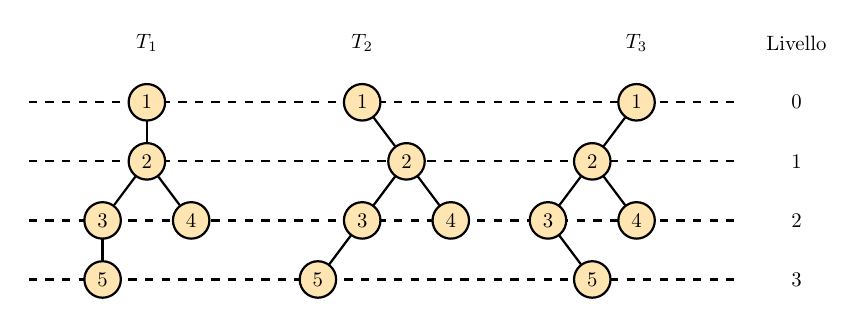
\begin{tikzpicture}[
	thick,
	scale=0.75,
	transform shape,
	level distance=1cm,
    each level/.style={sibling distance=1cm}
]
\tikzset{
    treenode/.style = {circle, draw=black, align=center,fill=ocra},
}

    \draw[dashed] (-2,0) -- (10,0);
    \draw[dashed] (-2,-1) -- (10,-1);
    \draw[dashed] (-2,-2) -- (10,-2);
    \draw[dashed] (-2,-3) -- (10,-3);

    \node (A) [treenode] {1}
    child { node[treenode] {2}
        child { node[treenode] {3}
            child {node[treenode] {5}}
        }
        child { node[treenode] {4} }
    }
    ;
    \node[above of=A] {$T_1$};
    \node (B) [treenode, right=3cm of A] {1}
    child[missing] {node {}}
    child { node[treenode](B2) {2}
        child { node[treenode] {3}
            child {node[treenode] {5}}
            child[missing] {node {}}
        }
        child { node[treenode] {4} }
    }
    ;
    \node[above of=B] {$T_2$};
    \node (C) [treenode, right=4cm of B] {1}
    child  { node[treenode] (C2) {2}
        child { node[treenode] {3}
            child[missing] {node {}}
            child {node[treenode] {5}}
        }
        child { node[treenode] {4} }
    }
    child[missing] {node {}}
    ;
    \node[above of=C] {$T_3$};
    \node at (11, 1) {Livello};
    \node at (11, 0) {0};
    \node at (11, -1) {1};
    \node at (11, -2) {2};
    \node at (11, -3) {3};
\end{tikzpicture}
\end{document}